\documentclass[11pt,a4paper]{article}

\usepackage{adjustbox}
\usepackage{algorithm}
\usepackage{algorithmic}
\usepackage{amsmath}
\usepackage{amssymb}
\usepackage{amsthm}
\usepackage{amsfonts}
\usepackage{afterpage}
\usepackage{blindtext}
\usepackage[font=footnotesize,labelfont=bf]{caption}
\usepackage{hyperref}
\usepackage[english]{babel}
\usepackage{bbm}
\usepackage{bigints}
\usepackage{bm}
\usepackage{cite}
\usepackage{color}
\usepackage{float}
\usepackage[left=2cm,right=2cm,top=2cm,bottom=2cm]{geometry}
\usepackage{graphicx}
\usepackage[utf8]{inputenc}
\usepackage{mathtools}
\usepackage{mdframed}
\usepackage{pgfplots} 
\usepackage{subfigure}
\usepackage{stmaryrd}
\usepackage{textcomp}
\usepackage{tikz}
\usepackage{url}
\renewcommand{\proofname}{Proof}
\theoremstyle{plain}
\newtheorem{monTheoNumrote}{Théorème}[section] % Environnement numéroté en fonction de la section
\newtheorem*{monTheoNonNumerote}{Théorème}  % Environnement non numéroté
\newtheorem{The}{Theorem}[section]
\newtheorem*{The*}{Theorem}
\newtheorem{Prop}{Proposition}[section]
\newtheorem*{Prop*}{Proposition} 
\newtheorem{Cor}{Corollary}[section]
\newtheorem*{Cor*}{Corollary}
\newtheorem{Conj}{Conjecture}[section]
\newtheorem{Lem}{Lemma}[section]
\renewcommand{\qed}{\unskip\nobreak\quad\qedsymbol}%
\numberwithin{equation}{section} % Numérote les équations section.numéro.
\theoremstyle{definition}
\newtheorem{Def}{Definition}[section]
\newtheorem{Rem}{Remark}[section]
\newtheorem*{Rem*}{Remark}
\newtheorem*{Lem*}{Lemma}
\newtheorem{Que}{Question}
\newcommand{\enstq}[2]{\left\{#1\mathrel{}\middle|\mathrel{}#2\right\}}
\newcommand{\Lp}[2]{L^#1(#2)}
\newcommand{\Sob}[3]{W^{#1,#2}(#3)}
\newcommand{\Rd}[0]{\mathbb{R}^d}
\newcommand{\RN}[0]{\mathbb{R}^N}
\newcommand{\Rn}[0]{\mathbb{R}^n}
\newcommand{\norm}[1]{\left\|#1\right\|}
\newcommand{\sinc}[0]{\textup{sinc}}
\newcommand{\functionDef}[5]{\begin{array}{lllll}
#1 & : & #2 & \longrightarrow & #3 \\
 & & #4 & \longmapsto &\displaystyle #5 \\
\end{array}}
\newcommand{\Theautorefname}{Theorem}
\newcommand{\Propautorefname}{Proposition}
\newcommand{\Corautorefname}{Corollary}
\newcommand{\Lemautorefname}{Lemma}
\newcommand{\Defautorefname}{Definition}
\newcommand{\N}{\mathbb{N}}
\newcommand{\Z}{\mathbb{Z}}
\newcommand{\D}{\mathbb{D}}
\newcommand{\R}{\mathbb{R}}
\newcommand{\A}{\mathcal{A}_{a,b}}
\newcommand{\Crad}{C^\infty_{c,rad}(B)}
\newcommand{\Lrad}{L^2_{rad}(B)}
\newcommand{\Lradab}{L^2_{rad}(\mathcal{A}_{a,b})}
\newcommand{\duality}[2]{\left\langle #1,#2\right\rangle}
\newcommand{\Hrad}{H^1_{rad}(B)}
\newcommand{\Hzrad}{H^1_{0,rad}(B)}
\newcommand{\rmin}{\delta_{\min}}
\newcommand{\rmax}{\delta_{\max}}
\newcommand{\corr}{\gamma}
\newcommand{\question}[1]{\begin{Que} \ 
#1
\end{Que}}
\newcommand{\abs}[1]{\left\lvert #1 \right\rvert}
\newcommand{\CL}[2]{\textup{CL}\left(\enstq{#1}{#2}\right)}
\newcommand{\Script}[1]{`\texttt{#1}`}
\newcommand{\espace}{\text{ }\qquad} 
\newcommand{\loc}{\text{loc}}
\newcommand{\SL}{\textup{SL}\hspace{1.5pt}}
\newcommand{\DL}{\textup{DL}\hspace{1.5pt}}
\newcommand{\fp}{\underset{\varepsilon \to 0}{\textup{f.p.}}}
\newcommand{\scalProd}[2]{\left(#1|#2\right)}
\newcommand{\toDo}[1]{{\color{red}#1}}
\newcommand{\bs}[1]{\boldsymbol{#1}}
\newcommand{\varInRange}[4]{(#1_{#2})_{#3 \leq #2 \leq #4}}
\newcommand{\from}{\colon}
\newcommand{\Cinf}{C^{\infty}}
\newcommand{\isdef}{\mathrel{\mathop:}=}
\newcommand{\defis}{=\mathrel{\mathop:}}

\renewcommand{\algorithmicrequire}{\textbf{Inputs:}}
\renewcommand{\algorithmicensure}{\textbf{Outputs:}}

\pgfplotsset{compat=1.13}
\title{Mini-projet : Modélisation de la conductivité thermique du laiton}
\author{Sujet proposé par Martin Averseng : martin.averseng@gmail.com}
\begin{document}
\maketitle

\begin{figure}
\begin{center}
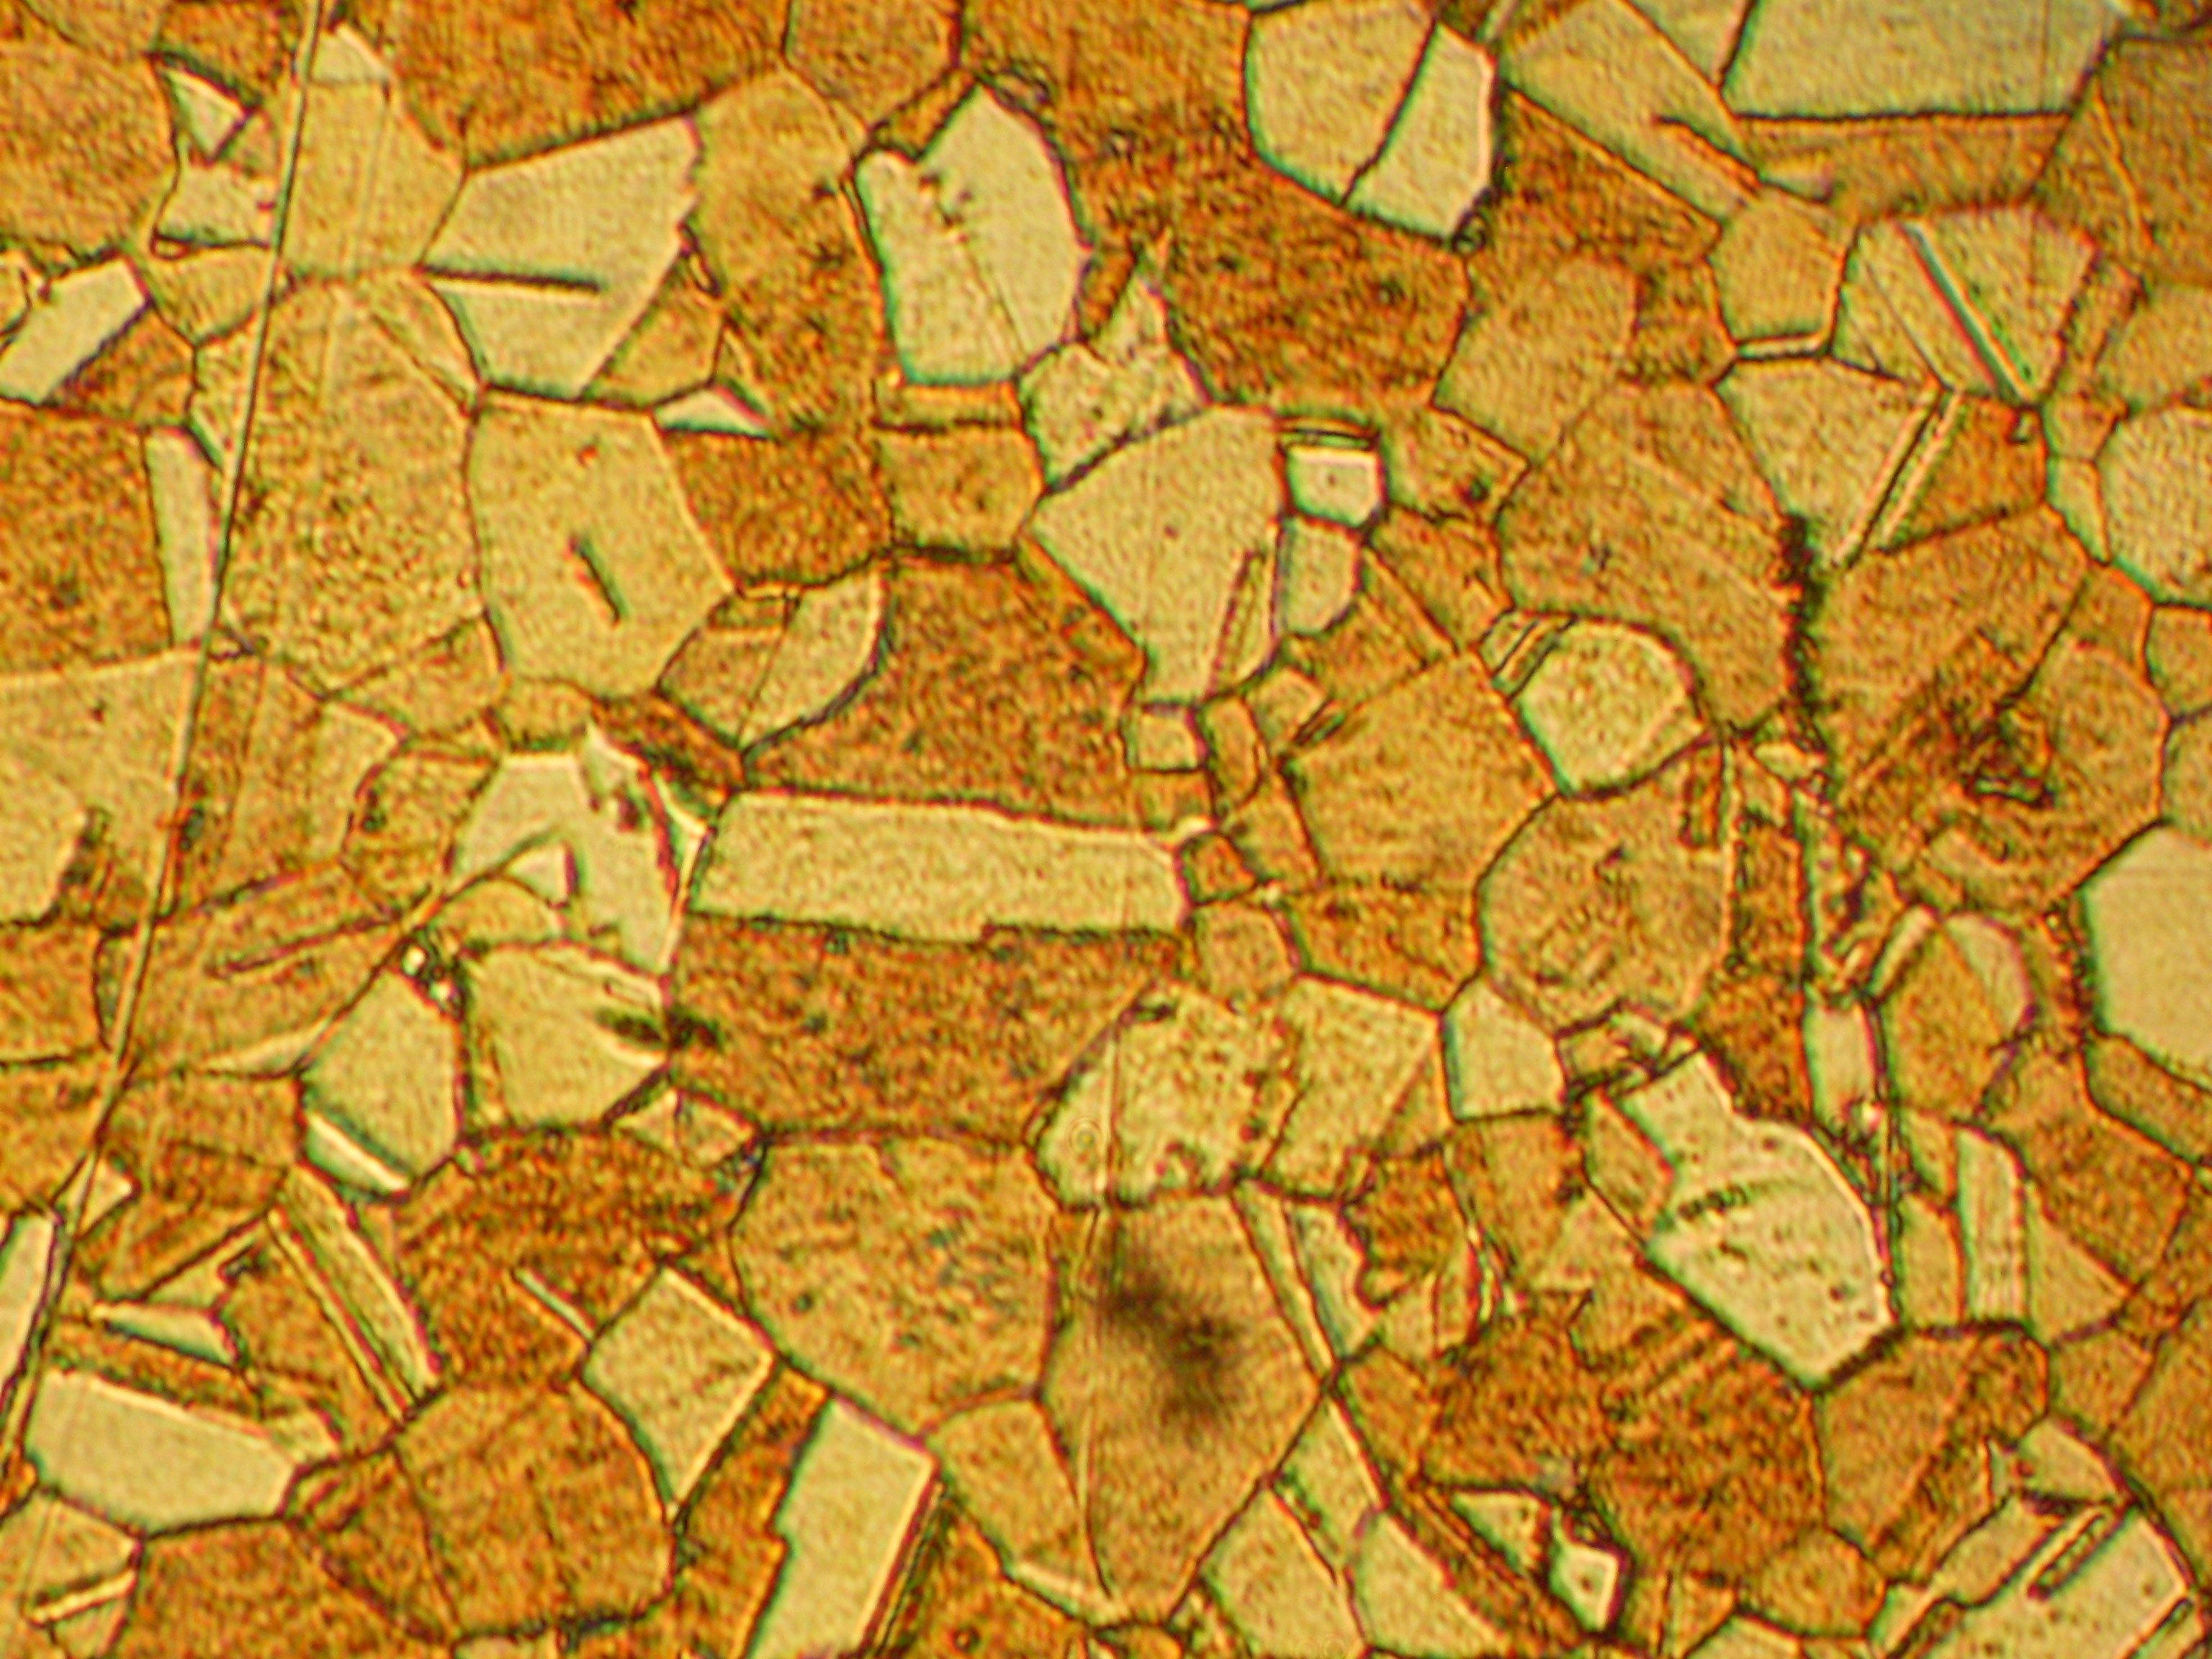
\includegraphics[width=0.5\textwidth]{LaitonMicrostruct.jpg} 
\end{center}
\caption{Micrographie d'un échantillon de laiton. On peut y voir des grains de cuivre et de zinc, formant deux phases solides. }
\end{figure}

On s'intéresse dans ce projet à la modélisation des transferts de chaleur dans un matériau composite tel que le laiton (alliage de cuivre et de zinc). On souhaite produire une simulation des transferts de chaleurs du  matériau initialement à température ambiante et soudainement placé dans un four chaud. On rappelle que dans un matériau occupant un domaine $\Omega$ supposé régulier, de conductivité thermique inhomogène donnée par le tenseur $a(x)$, soumis à une température fixée $u_{ext}(x,t)$ sur la frontière de son domaine $\partial \Omega$, et soumis à une source de chaleur $g(x,t)$ dans le domaine $\Omega$, la température $u$ vérifie l'équation aux dérivées partielles suivante : 

\begin{equation}
\left\{
\begin{array}{rll}
\dfrac{\partial u}{\partial t}(t,x) - \nabla \cdot (a(x)\cdot  \nabla u (t,x)) &= g(x,t) & \text{ dans } \Omega,\\
u(x,t) &= u_{ext}(x,t) & \text{ sur } \partial \Omega, \\
u(x,0) &= u_0(x) & \text{ sur } \Omega,
\end{array}\right.
\label{EqChaleurInhomogene}
\end{equation}
où $u_0 \in L^2(\Omega)$ est la température initiale. On fait l'hypothèse que $g \in L^2(\mathbb{R}^+,L^2(\Omega))$ et que  le tenseur (d'ordre égal à la dimension) des conductivités $a(x)$ a ses coefficients bornés et vérifie l'hypothèse d'ellipticité uniforme suivante : \\
\begin{equation}
\label{CoerciviteUniforme}
\text{Il existe deux constantes $c>0$ et $C>0$ telles que $\forall x,\xi \in \mathbb{R}^d$, $ c \norm{\xi}^2 \leq \xi^T a(x) \xi \leq C \norm{\xi}^2$.}
\end{equation}


\section{Mise sous forme variationnelle}

Cette section est dédiée à mettre le problème sous forme variationnelle, et démontrer son caractère  bien posé. Nous conseillons d'omettre les questions les plus théoriques (notées avec une étoile) dans un premier temps. 
On commence par se ramener à une condition de Dirichlet homogène. Pour cela, on définit l'espace suivant : \\


\begin{Def} L'espace $H^{1/2}(\partial\Omega)$ est l'image de l'espace $H^1(\Omega)$ par l'application trace $\gamma_0$ au bord de $\Omega$. 
\end{Def}
On admet le résultat de relèvement suivant :
\begin{The}
Il existe une application linéaire continue $R_0 : H^{1/2}(\partial \Omega) \to H^1(\Omega)$  vérifiant $\gamma_0 \circ R_0 = Id_{\partial \Omega}$. Une telle application est appelée un relèvement continu de $H^{1/2}(\partial \Omega)$ dans $H^1(\Omega)$. 
\end{The}

\question{(*) Soit $X$ et $Y$ deux espaces de Banach et $L$ une application linéaire continue de $X \to Y$. Soit $T>0$ et $u \in C^k([0,T],X)$. Montrer que $Lu \in C^k([0,T],Y)$ (on montrera le résultat pour $k = 0$ et on procédera par récurrence). }

\question{Indiquer comment se ramener, pour l'étude du problème (\ref{EqChaleurInhomogene}), à un problème avec conditions de Dirichlet homogènes :
\begin{equation}
\left\{
\begin{array}{rll}
\dfrac{\partial \tilde{u}}{\partial t}(t,x) - \text{div}(a(x)\cdot  \nabla  \tilde{u} (t,x)) &= f(x,t) + g(x,t) & \text{ dans } \Omega,\\
\tilde{u}(x,t) &= 0 & \text{ sur } \partial \Omega.\\
\tilde{u}(x,0) &= \tilde{u}_0(x) & \text{ sur } \Omega	
\end{array}\right.
\label{EqChaleurInhomogene2}
\end{equation}
Où $f(x,t) = -\dfrac{\partial U}{\partial t} + \text{div}(a(x)\nabla U)$, $\tilde{u}(x,t) = u(x,t) - U(x,t)$ et où $U(x,t) = R u_{ext}(x,t)$, $R$ étant un relèvement continu de $H^{1/2}(\partial \Omega)$ dans $H^1(\Omega)$.}

\question{Montrer que pour toute fonction $h \in H^1_0(\Omega)$, les distributions $h$ et $\text{div}(a(x)\nabla h)$ s'identifient à des formes linéaires sur $H^1_0(\Omega)$. \\
(Par définition, pour montrer qu'une distribution $v$ définie  s'identifie à une forme linéaire sur $H^1_0(\Omega)$, il faut montrer que 
\[ \duality{v}{\varphi} \leq C \norm{\varphi}_{H^1_{0}(\Omega)},\]
pour toute fonction test $\varphi$)}
Par la suite, on note $H^{-1}(\Omega)$ l'espace dual de $H^1_0(\Omega)$. Puisque c'est le dual d'un espace de Hilbert, c'est aussi un espace de Hilbert. La question précédente montre donc que $H^1_0(\Omega) \subset H^{-1}(\Omega)$ et que l'application linéaire $h \mapsto \text{div}(a(x) \nabla h)$ est un élément de $\mathcal{L}(H^1_0(\Omega),H^{-1}(\Omega))$. Pour toute forme linéaire $T \in H^{-1}(\Omega)$, on notera $\duality{T}{v}_{H^{-1}\times H^1_0(\Omega)}$ la valeur prise par T en $v$.  

\question{(*) Montrer que si $u_{ext}(x,t)$ est $C^1([0,T],H^{1/2}(\partial \Omega)$), alors $f$ est $C([0,T],H^{-1}(\Omega))$. }
Par la suite, on oubliera les "tilde" pour alléger les notations. Comme pour tout $t \in [0,T]$, $f(t)$ est un élément de $H^{-1}(\Omega)$, on peut définir $\duality{f(t)}{\varphi}_{H^{-1}\times H^1_0(\Omega)}$ pour toute fonction $\phi \in H^1_0(\Omega)$ comme la valeur de la forme linéaire $f(t)$ prise en $\varphi$. 

On introduit le problème variationnel suivant :
\begin{equation}\left\{\begin{array}{rlll}
\dfrac{d}{dt}\duality{u(t)}{v}_{L^2(\Omega)} + \displaystyle\int_{\Omega} \duality{a(x) \nabla u} {\nabla v} &= \duality{f(t)}{v}_{H^{-1}\times H^1_{0}(\Omega)} +\duality{g(t)}{v}_{L^2(\Omega)}  & \forall v \in H^1_0(\Omega), & \forall t \in ]0,T[ \\
u(x,0) &= u_0(x) 
\end{array}\right.
\label{FormeVaritionnelle}
\end{equation}

On souhaite démontrer que ce problème possède une unique solution. Pour cela, on s'appuie sur le théorème 8.2.3 du polycopié de cours MAP 431 (Analyse numérique et optimisation, Grégoire Allaire, disponible en ligne sur la page du cours, page 241 de la deuxième édition).

\question{Dans cette question, on renforce les hypothèses sur $f$, à savoir qu'il existe une fonction notée $h \in L^2([0,T],L^2(\Omega))$ telle que $\duality{f(t)}{\cdot}_{H^{-1}\times H^1_{0}(\Omega)} = \duality{h(t)}{\cdot}_{L^2(\Omega)}$ pour presque tout $t \in ]0,T[$ (en d'autres termes, on suppose $f\in L^2([0,T],L^2(\Omega))$ Montrer qu'alors les hypothèses du théorème mentionné ci-dessus sont toutes satisfaites, et en déduire que le problème variationnel (\ref{FormeVaritionnelle}) a une unique solution. }

On note $u_k$ une base hilbertienne de vecteurs propres dans $H^1_{0}(\Omega)$ pour la forme bilinéaire $a : (u,v) \mapsto \int_{\Omega} \duality{a(x) \nabla u} {\nabla v}$ et  
\[ \beta_k(t) = \duality{f(t)}{u_k}_{H^{-1}\times H^1_{0}(\Omega)},\]


En étudiant la preuve du théorème, on remarque que si l'hypothèse précédente sur $f$ n'est pas vérifiée, le résultat est toujours vrai à condition de démontrer que :
\[\sum_{k=1}^{+\infty} \int_{0}^T\abs{\beta_k(s)}^2ds < +\infty.\]
\question{(*) Soit $n \in \mathbb{N^*}$ et $t \in [0,T]$. On pose 
\[\gamma_n(t) =  \sqrt{\sum_{k=1}^n \abs{\beta_k(t)}^2},\]
et on introduit 
\[ v_n(t) = \dfrac{1}{\gamma_n(t)} \sum_{k=1}^n \beta_k(t) u_k\]
Vérifier que $\norm{v_n(t)}_{H^1_0(\Omega)} = 1$. En appliquant $f(t)$ à $v_n(t)$, prouver que $\gamma_n(t) \leq \norm{f(t)}_{H^{-1}}$.
En déduire que 
\[\sum_{k=1}^{n} \int_{0}^T\abs{\beta_k(s)}^2ds < \norm{f}_{L^2([0,T],H^{-1}(\Omega))}^2.\]
Conclure.}

\section{Approximation numérique par éléments finis}

On propose de résoudre numériquement l'équation (\ref{FormeVaritionnelle}) par la méthode des éléments finis en espace, associée à un schéma aux différences finies en temps, de type implicite ($\theta = 1$). On va voir que cette méthode s'adapte bien au cas où les inhomogénéités du matériau sont assez grandes devant la taille du maillage, mais devient inefficace dans le cas contraire. 

\subsection{Semi-discrétisation en espace}

Soit $V_h$ un sous-espace de dimension finie de $H^1_0(\Omega)$ et $B_h = (e_1,...,e_{nddl})$ une base de $V_h$. On introduit le problème variationnel discrétisé :
\begin{equation}\left\{\begin{array}{rlll}
\dfrac{d}{dt}\duality{u_h(t)}{v_h}_{L^2(\Omega)} + a(u_h(t),v_h) &= \duality{f(t)}{v_h}_{H^{-1}\times H^1_{0}(\Omega)}+  \duality{g(t)}{v_h}_{L^2(\Omega)} & \forall v_h \in V_h, & \forall t \in ]0,T[ \\
u_h(0) &= u^0_h,
\end{array}\right.
\label{FormeVaritionnelleDiscrete}
\end{equation}
où l'inconnue $u_h$ est cherchée comme une fonction de $t$ à valeur dans $V_h$, et où $u^0_h$ est une approximation de $u_0$ dans $V_h$.
\question{Montrer que si $u_h$ est solution de ce problème variationnel, le vecteur de ses coordonnées $U_h(t)$ dans la base $B_h$ vérifie un système d'équations différentielles du type
\begin{equation}
\left\{\begin{array}{rl}
\mathcal{M} \dfrac{d U_h}{dt} + \mathcal{K}U_h &= b_h(t)\\
U_h(0) &= U^0_h ,
\end{array}\right.
\end{equation}
où $U^0_h$ est la matrice des coordonnées de $u^0_h$ dans $B_h$. Donner l'expression de la matrice de masse $\mathcal{M}$, de la matrice de rigidité $\mathcal{K}$ et du second membre $b_h(t)$. Montrer que ce problème à une solution unique dans $C^1([0,T],V_h)$.}

\subsection{Discrétisation totale espace-temps}

On considère un sous-espace de dimension finie $V_h$ de $H^1_0(\Omega)$, et on se donne une base $(e_1,e_2,...,e_{nddl})$ d'éléments de $V_h$. On coupe l'intervalle $]0,T[$ en $n$ sous-segments $]0,t_1[, ]t_1,t_2[, ..., ]t_{n-1},T[$ où $t_i$ est donné par $i\Delta t$ avec $\Delta t = \frac{T}{n}$. On note $(U^i)_{0 \leq i \leq n}$ la suite récurrente telle que $U^0$ est une approximation de $u_0$ sur $V_h$, et  $U^{i+1}$ est défini à partir de $U^i$ par le schéma d'Euler implicite en temps associé à la discrétisation spatiale par éléments finis. 
\begin{equation}
\left(\mathcal{M} + \Delta t\mathcal{K}\right)U^{i+1} = \left( U^i + \Delta t b(t^{i+1})\right)
\label{SchemaImplicite}
\end{equation}

\question{Démontrer la stabilité inconditionnelle de ce schéma.}
Nous allons maintenant implémenter numériquement ce schéma pour un problème en dimension $1$, $\Omega =  [0,1]$ sur scilab, pour une approximation par éléments finis $\mathbbm{P}^1$. On introduit un maillage uniforme de l'intervalle $[0,1]$ avec les notations suivantes : pour $i \in \llbracket 0, \text{nddl}+1 \rrbracket$, $x_i = i h$ où $h = \dfrac{1}{\text{nddl+1}}$. L'espace d'approximation sera donné par 
\[ V_{h} = \enstq{v \in C^0([0,1])}{v \text{ est affine sur chaque segment} [x_i, x_{i+1}] \text{ et } v(0) = v(1) = 0}.\]
On choisira comme base de l'espace $V_h$ la base usuelle des éléments finis $\mathbbm{P}^1$, c'est-à-dire que pour tout $i \in \llbracket 1,\text{nddl}\rrbracket$, la i-ième fonction de base $\phi_i$ est nulle en tous les $x_j$ sauf pour $j = i$ où elle prend la valeur $1$. 

\question{Donner l'expression explicite de la matrice de masse (de taille nddl$\times$nddl). Ecrire une procédure \texttt{Silab} ayant pour syntaxe \texttt{M$=$assemble\_masse(nddl)} qui renvoie la matrice creuse \texttt{M} égale à la matrice de masse du problème.}

\question{Vérifier que la matrice de rigidité est donnée par 
\begin{align*}
& \mathcal{K}_{i,i-1} = \mathcal{K}_{i-1,i} = \dfrac{-1}{h^2}\int_{(i-1)h}^{ih}a(x)dx &\text{ pour tout } i\in \llbracket 2,\text{nddl}\rrbracket\\ 
& \mathcal{K}_{i,i} = \dfrac{1}{h^2}\int_{(i-1)h}^{(i+1)h}a(x)dx &\text{ pour tout } i\in \llbracket 1,\text{nddl}\rrbracket\\
&\mathcal{K}_{i,j} = 0 &\text{ si } |i-j| \geq 2
\end{align*}
}
En général, il n'est pas possible de connaître explicitement la valeur des termes de la matrice de rigidité. En revanche, lorsque la conductivité thermique $a$ varie peu au sein de chaque segment $[x_i,x_{i+1}]$, on peut approcher les valeurs par des méthodes de quadrature numérique. Ici, sans entrer dans les détails, on utilisera l'approximation suivante
\[\int_{a}^{b}f(t)dt \approx \dfrac{b-a}{6}\left(f(a) + 4f\left(\dfrac{a+b}{2}\right) + f(b) \right)\]
\question{Ecrire une procédure \texttt{Scilab} ayant pour syntaxe \texttt{K$=$assemble\_rigidite(nddl,func\_a)} qui renvoie la matrice creuse \texttt{K} égale à la matrice de rigidité du problème. La variable \texttt{func\_a} transporte l'information sur la conductivité thermique $a$ pour calculer les intégrales dans la définition de \texttt{K}. On pourra par exemple passer en argument le nom d'une procédure \texttt{Scilab} ayant pour syntaxe \texttt{r}$=$\texttt{func\_a(x)} qui renvoie la valeur \texttt{r} de la conductivité thermique au point \texttt{x}. }

Pour assembler le second membre, on fera l'approximation que $g(x,t)$ est bien approché par sa projection sur le maillage 
\[g_h(t) = \sum_{i=1}^{\text{nddl}}g(x_i,t)\phi_i(x).\]
On notera $G_h(t)$ le vecteur des coordonnées de $g_h(t)$ dans $V_h$.    
\question{Montrer que l'on peut choisir $U_{ext}(x,t) = u_{ext}(0,t)\phi_0(x) + u_{ext}(1,t) \phi_{\text{nddl}+1}(x)$ (où les fonctions $\phi_0$ et $\phi_{\text{nddl}+1}$ sont les fonctions éléments finis usuelles au bord du domaine, c'est-à-dire les fonctions continues affines sur chaque $[x_i,x_{i+1}]$ pour tout $i \in \llbracket 0, \text{nddl}\rrbracket$, nulles partout sauf respectivement en $x_0$ et $x_{\text{nddl}+1}$ où elles sont égales à $1$). Montrer qu'avec ce choix, on trouve l'expression suivante pour l'entrée $i$ du vecteur $b$ :
\begin{multline*}
b_i(t) = \left(\mathcal{M}G_h(t)\right)_i -\dfrac{\partial u_{\text{ext}}}{\partial t}(0,t)\int_{\Omega} \phi_{0}\phi_i - \dfrac{\partial u_{\text{ext}}}{\partial t}(1,t)\int_{\Omega} \phi_{\text{nddl}+1}\phi_{i}\\ 
- u_{\text{ext}}(0,t) \int_{\Omega}a(x) \nabla \phi_0 \nabla \phi_i - u_{\text{ext}}(1,t)\int_{\Omega}a(x) \nabla \phi_{\text{nddl}+1} \nabla \phi_i
\end{multline*}}
En déduire que 
\begin{align*}
& b_{1}(t) = \left(\mathcal{M}G_h(t)\right)_1 -\dfrac{h}{6}\dfrac{\partial u_{\text{ext}}}{\partial t}(0,t) + \dfrac{1}{h^2} u_{\text{ext}}(0,t)\int_{0}^h a(x)dx\\ 
& b_i(t) = \left(\mathcal{M}G_h(t)\right)_i & \text{Pour } i \in \llbracket 2, \text{nddl}-1\rrbracket\\
& b_{\text{nddl}}(t) = \left(\mathcal{M}G_h(t)\right)_{\text{nddl}} -\dfrac{h}{6}\dfrac{\partial u_{\text{ext}}}{\partial t}(1,t) + \dfrac{1}{h^2} u_{\text{ext}}(1,t)\int_{1-h}^1 a(x)dx\\
\end{align*}
\question{Ecrire une procédure \texttt{Scilab} ayant pour syntaxe \\ \texttt{b} $=$ \texttt{assemble\_secondMembre(nddl,t,func\_a,func\_u,func\_du,Gh,M)} qui assemble le second membre (creux) correspondant au problème avec le choix décrit dans la question précédente. Les arguments \Script{func\_u} et \Script{func\_du} contiennent l'information sur la température imposée aux deux bords et sa dérivée.}

\question{Ecrire une procédure qui calcule numériquement la solution de (\ref{EqChaleurInhomogene}).}
Pour valider le code, on choisit une fonction arbitraire $u(t,x)$ et une fonction quelconque $a(x)$ (vérifiant les hypothèses), et on calcule le second membre $g$ et la température imposée $u_{\text{ext}}$ qui correspondent, et on lance le code précédent sur ces données pour vérifier que la solution obtenue est proche de la solution exacte.

\question{ Calculer la source $g$, la température $u_{ext}(x,t)$ et la condition initiale $u_0(x)$ pour lesquelles la solution $u$ est donnée $u(x,t)=\sin(t)\cos(x)$ avec $a(x) = 1+x$.}

\question{En notant $U_h(t)$ le vecteur des coordonnées de la solution approchée $u_h$ sur le maillage, $\pi_h u(x,t)$ la projection de la solution exacte sur le maillage, $\pi_hU(t)$ le vecteur de ses coordonnées dans la base des éléments finis, et $E_h(t) = \pi_h U - U_h$ montrer que 
\[\norm{u_h(x,t) - \pi_h u(x,t)}_{H^1_0(\Omega)} = \sqrt{\left(\mathcal{K}_0E_h\right)\cdot E_h}\]
où $\mathcal{K}_0$ serait la matrice de rigidité du problème pour $a(x) \equiv 1$. Tracer l'évolution de l'erreur mesurée en norme $H^1_0$ en fonction du temps pour différents pas de discrétisation $h$.}




\section{Homogénéisation}

Nous sommes maintenant capables de traiter le problème suivant : soit un paramètre $\varepsilon$, et soit $a_{\varepsilon}$ définie pour $x\in  [0,1]$ par : 
\[a_{\varepsilon}(x) = \alpha\left(\dfrac{x}{\varepsilon}\right) \]
Où $\alpha$ est la fonction $1$-périodique sur $\mathbb{R}$ dont la restriction sur $[0,1]$  a la forme suivante :
\[\alpha(x)|_{[0,1]} = \alpha_1\mathbbm{1}_{0<x<1/2}  +\alpha_2 \mathbbm{1}_{1/2<x<1}.\]
Les constantes positives $\alpha_1$ et $\alpha_2$ représentent la conductivité du cuivre et du zinc. 
La figure suivante montre une représentation de $a_\varepsilon$ sur $[0,1]$ pour $\varepsilon = 0.15$. 

\begin{figure}[width = 0.3\textwidth; H]
\centering
\begin{adjustbox}{width=0.7\textwidth}
% This file was created by matlab2tikz.
%
%The latest updates can be retrieved from
%  http://www.mathworks.com/matlabcentral/fileexchange/22022-matlab2tikz-matlab2tikz
%where you can also make suggestions and rate matlab2tikz.
%
\definecolor{mycolor1}{rgb}{0.00000,0.44700,0.74100}%
%
\begin{tikzpicture}

\begin{axis}[%
width=4.521in,
height=3.323in,
at={(0.758in,0.724in)},
scale only axis,
xmin=-0.2,
xmax=1.2,
xlabel={$x$},
ymin=0.5,
ymax=2.5,
ytick={1,2},
yticklabels = {$\alpha_1$,$\alpha_2$},
ylabel={$a_{\varepsilon}(x)$},
axis background/.style={fill=white}
]
\addplot [color=mycolor1,solid,line width=3.0pt,forget plot]
  table[row sep=crcr]{%
0	1\\
0.01	1\\
0.02	1\\
0.03	1\\
0.04	1\\
0.05	1\\
0.06	1\\
0.07	1\\
0.08	2\\
0.09	2\\
0.1	2\\
0.11	2\\
0.12	2\\
0.13	2\\
0.14	2\\
0.15	1\\
0.16	1\\
0.17	1\\
0.18	1\\
0.19	1\\
0.2	1\\
0.21	1\\
0.22	1\\
0.23	2\\
0.24	2\\
0.25	2\\
0.26	2\\
0.27	2\\
0.28	2\\
0.29	2\\
0.3	1\\
0.31	1\\
0.32	1\\
0.33	1\\
0.34	1\\
0.35	1\\
0.36	1\\
0.37	1\\
0.38	2\\
0.39	2\\
0.4	2\\
0.41	2\\
0.42	2\\
0.43	2\\
0.44	2\\
0.45	1\\
0.46	1\\
0.47	1\\
0.48	1\\
0.49	1\\
0.5	1\\
0.51	1\\
0.52	1\\
0.53	2\\
0.54	2\\
0.55	2\\
0.56	2\\
0.57	2\\
0.58	2\\
0.59	2\\
0.6	1\\
0.61	1\\
0.62	1\\
0.63	1\\
0.64	1\\
0.65	1\\
0.66	1\\
0.67	1\\
0.68	2\\
0.69	2\\
0.7	2\\
0.71	2\\
0.72	2\\
0.73	2\\
0.74	2\\
0.75	1\\
0.76	1\\
0.77	1\\
0.78	1\\
0.79	1\\
0.8	1\\
0.81	1\\
0.82	1\\
0.83	2\\
0.84	2\\
0.85	2\\
0.86	2\\
0.87	2\\
0.88	2\\
0.89	2\\
0.9	1\\
0.91	1\\
0.92	1\\
0.93	1\\
0.94	1\\
0.95	1\\
0.96	1\\
0.97	1\\
0.98	2\\
0.99	2\\
1	2\\
};
\end{axis}
\end{tikzpicture}%
\end{adjustbox}
\caption{Représentation de la conductivité $a_\varepsilon$ sur $[0,1]$ pour $\varepsilon = 0.15$, pour $\alpha_1 = 1$ et $\alpha_2 = 2$.}
\end{figure}

Comme la géométrie est ici fixée à $[0,1]$, $\varepsilon$ représente le rapport entre la taille caractéristique des inhomogénéités du matériau et la longueur de l'échantillon de laiton considéré. Ainsi, plus $\varepsilon$ est petit, plus on modélise un "gros" morceau de laiton. En pratique, on s'intéresse bien sûr à des morceaux de laitons bien plus gros que la taille caractéristique des inhomogénéités, donc on souhaite résoudre le problème lorsque $\varepsilon$ est très petit. 

On pose $u_l = 1$ et $u_r = 10$. On introduit le problème stationnaire suivant : 
\[
\left\{
\begin{array}{rl}
&-(a_{\varepsilon}u_{\varepsilon}')'(x) = 0 \text{ pour tout $x \in [0,1]$}\\
&u(0) = u_l, u(1) = u_r
\end{array}
\right.
\]

\question{Déterminer la solution explicite de ce problème. Utiliser les fonctions codées précédemment pour la calculer numériquement. En faisant varier $\varepsilon$ tout en gardant le maillage constant, que remarquez vous ? Pouvez-vous espérer obtenir une bonne approximation numérique de la solution pour $\varepsilon \approx 10^{-5}$, qui est l'ordre de grandeur de $\varepsilon$ pour une barre d'un mètre de laiton ? }

Nous allons montrer que lorsqu'$\varepsilon$ tend vers $0$, la solution du problème converge dans $L^2$ vers la solution d'une équation aux dérivées partielles facile à résoudre numériquement. 

\question{Soit $<a> = \displaystyle\int_{0}^1 a(x)$. Soit $u \in L^2([0,1])$, montrer que
\[ \lim_{\varepsilon \to 0}\int_0^u a_{\varepsilon}(x) u(x)dx = <a> \int_{0}^1 u(x) dx\]  }

\question{Montrer que la solution du problème }

\end{document}

